\documentclass[dvipdfmx,a4paper,twocolumn,10pt]{jarticle}
\usepackage[dvipdfmx]{graphicx}
\usepackage{csn-abst}   % CSN style
\usepackage{amsmath}
\usepackage{multicol}
\usepackage{multirow}
\usepackage[hang,labelsep=period]{caption}  
\usepackage{fancyhdr}
\usepackage{lastpage}
\usepackage{longtable}
\usepackage{supertabular}
\usepackage{booktabs}
\usepackage{subfigure}
\usepackage{algorithmic}
\usepackage{algorithm}


% \title{長いタイトルは途中で改行を入れると\\好きなところで折り返せる} % 卒論題目(2行)
\title{テクニカル指標の組み合わせによるトレーディングアルゴリズムの提案}% 卒論題目
\author{オンコン マハルク ラフマン}       % 学生氏名
\studentnumber{202C1032}       % 学生番号
\course{ソフトウェアデザイン}  % コース名
%\course{情報通信ネットワーク}  % コース名
%\course{コンピュータ工学}  % コース名
\supervisor{藤原 暁宏}          % 指導教員氏名
\year{2023}                    % 年度

\begin{document}
\maketitle

\section{はじめに}
近年,金融分野で数学や情報科学を応用したフィナンシャルテクノロジーが注目を浴びている.
その中でも,株取引においては,アルゴリズムを用いて自動的に注文を判断し実行するアルゴリズム取引が活発に行われている\cite{python_trade}.

本研究では複数のテクニカル指標を組み合わせたアルゴリズムをトレーディングツールを用いて検証し,
有効な組み合わせを提案することを目指す.提案アルゴリズムは,
実際の東証の株価データを用いたバックテストを通じて,有効性の検証を行う.

\section{テクニカル指標}
アルゴリズムトレーディングで用いられるテクニカル指標は数多く存在するが,ここでは本研究で用いる主なテクニカル指標を2つ説明する.

\begin{itemize}

    \item MACD (Moving Average Convergence and Divergence)
    
    短期と中期の移動平均線がどちらも横ばいか上向きであり,短期移動平均線を中期移動平均線が下から上に突き抜ける買いのタイミングをゴールデンクロスと呼ぶ.MACDはこのゴールデンクロスを更に汎用的にしたテクニカル指標である.
MACDでは移動平均として,単純移動平均ではなく,直近の価格に比重をおく平滑移動平均を用いる.MACDは,
MACD(短期線と長期線の差),シグナル(MACDの平滑移動平均),ヒストグラム(MACDとシグナルの差)の3つの要素で構成されており,
MACDがシグナルを下から上へ突き抜けるというタイミングが買いのシグナルである.
\end{itemize}
\begin{itemize}
  \item ボリンジャーバンド (BB: Bollinger Band)
  
  移動平均線の上下に標準偏差を元に計算された3つのバンドという線を加えてたテクニカル指標である.
株価の変動はバンドの範囲内に収まることが多いと考えられており,ばらつきが多いほど標準偏差は大きくなるため,バンドの幅が広くなる方に値動きが大きくなると判断できる.
\end{itemize}


\section{提案トレーディングアルゴリズム}
本研究では以下の売買条件を組み合わせて取引を行う.以下の$tp$,$sl$は,利確,損切りを行うパーセンテージを表すパラメタであり,これらの値を変更して最適化を行う.

\begin{description}
\item[\textbf{購入条件:}]以下の購入条件の組み合わせにより,株を購入する.


\item[\textbf{(B1):}] MACDがシグナルを下から上へ突き抜ける.
\item[\textbf{(B2):}] 注目する日の終値が,BBの-2σを上から下へ突き抜ける.
\item[\textbf{(B3):}] 60日移動平均線の傾きが0以上である.
\item[\textbf{(B4):}] 注目する日の日経平均株価の長期線の傾きが0以上である.

\item[\textbf{売却条件:}]購入後,以下のいずれかの条件が成り立つとき,購入した株を売却する.

\item[\textbf{(S1):}] 株の始値が購入した株価より$tp$%以上である.
\item[\textbf{(S2):}] 株の始値が購入した株価より$sl$%以下である.

\end{description}

\section{実験結果と考察}
\begin{figure}[t]
  \centering
  \includegraphics[page=4,width=\linewidth,scale=0.5]{graph.png}
  \caption{実行結果}
  \label{fig:result}
 \end{figure}
 本研究では,提案アルゴリズムをpython3を用いたバックテスト環境であるBacktesting.pyに実装し,過去10年分の東証株価データに対して評価を行う.
 
 図\ref{fig:result}に各条件の組み合わせに対して得られた10年間の平均利益を示す.図\ref{fig:result}より,利益を求めるならば,「(B1)または(B2)」の条件が適しており,利益は下がるが勝率を求めるのならば「(B2)かつ(B4)」が適していることがわかる.

また,利確を行う$tp$は約107%が適しており,損切りを行う$sl$は約93%が適していることがわかる.
\section{まとめ}
本研究では複数のテクニカル指標を組み合わせたトレーディングアルゴリズムの提案とシミュレーションによる評価を行った.今後の課題としてここでは述べていない他のテクニカル指標を用いた検証や,AIを用いたトレーディングアルゴリズムの提案などが挙げられる.
\begin{thebibliography}{99}\small

\bibitem{python_trade} {
片渕, {Pythonでできる!株価データの分析}, 森北出版, 2023.}

\end{thebibliography}

\end{document}
